\documentclass[11pt]{article}

\def\chapitre{3}
\def\pagetitle{Fonctions usuelles.}

\input{/home/theo/MP2I/setup.tex}

\begin{document}

\input{/home/theo/MP2I/title.tex}

\thispagestyle{fancy}

\section{Fonction exponentielle.}

\begin{defi}{}{}
    La fonction \bf{exponentielle} est l'unique fonction $\exp:\R\to\R$ dérivable sur $\R$ et telle que
    \begin{equation*}
        \exp(0)=1\quad\nt{et}\quad\forall x\in\R,~\exp'(x)=\exp(x).
    \end{equation*}
\end{defi}

\begin{prop}{Faits.}{}
    \begin{enumerate}
        \item La fonction exp prend ses valeurs dans $]0,+\infty[$.
        \item Elle est strictement croissante sur $\R$.
        \item Elle a une tangente en 0 d'équation $y=x+1$. De plus,
        \begin{equation*}
            \forall x \in \R,~\exp(x)\geq x+1.
        \end{equation*}
    \end{enumerate}
\end{prop}

\begin{thm}{Propriété de morphisme de l'exponentielle.}{}
    \begin{center}
        \boxed{\forall x \in \R, ~ \forall y \in \R, \quad \exp(x+y)=\exp(x)\exp(y)},
    \end{center}
    Il découle de cette propriété que
    \begin{enumerate}
        \item $\forall x \in \R, ~ \exp(-x)=\exp(x)^{-1}$,
        \item $\forall x \in \R, ~ \forall y \in \R, ~ \exp(x-y)=\frac{\exp(x)}{\exp(y)}$,
        \item $\forall x \in \R, ~ \forall p \in \Z, ~ \exp(px)=\exp(x)^p$.
    \end{enumerate}
    \tcblower
    Ça ne sera démontré qu'en fin d'année.....
\end{thm}

\section{Logarithme népérien.}

La fonction $\exp$ est une bijection de $\R$ dans $]0,+\infty[$. Plus précisément, tout élément $y\in\R_+^*$ possède un unique antécédent par exp dans $\R$, que l'on va noter $\ln(y)$.

\begin{defi}{}{}
    On appelle \bf{logarithme népérien} la fonction $\ln:]0,+\infty[\to\R$, réciproque de l'exponentielle.
\end{defi}

\begin{center}
    \includegraphics*[scale=0.7]{graphe_logexp.png}
\end{center}

La réciprocité de $\ln$ et de $\exp$ implique notamment
\begin{center}
    \boxed{\forall x \in \R, ~ \ln(\exp(x))=x} \quad et \quad \boxed{\forall y \in ]0,+\infty[, ~ \exp(\ln(y))=y}.
\end{center}

\begin{prop}{}{}
    La fonction $\ln$ est dérivable sur $]0,+\infty[$ de dérivée la fonction inverse : $\forall y \in ]0,+\infty[,~\ln'(y)=\frac{1}{y}$.\\
    Le graphe a une tangente en 1 d'équation $y=x-1$. De plus,
    \begin{equation*}
        \forall x \in ]0,+\infty[,~\ln(x)\leq x-1.
    \end{equation*}
\end{prop}

\begin{prop}{Propriété du morphisme du logarithme.}{}
    \begin{equation*}
        \forall x \in \R^*_+,~\forall y \in \R^*_+,~\ln(xy)=\ln(x)+\ln(y).
    \end{equation*}
    Il découle de cette propriété que
    \begin{itemize}
        \item $\forall x \in \R^*_+,~\ln\left( \frac{1}{x} \right)=-\ln(x)$.
        \item $\forall p \in \Z,~\forall x \in \R_+^*,~\ln(x^p)=p\ln(x)$.
    \end{itemize}
\end{prop}

\begin{ex}{}{}
    Le logarithme de dix milliards, c'est grand comment ?
    \tcblower
    On a $\ln(10^{10})=10\ln(10)$ c'est approximativement 23.
\end{ex}

\begin{defi}{}{}
    Soit $a\in\R^*_+\setminus\{1\}$. La fonction \bf{logarithme en base $a$}, notée $\log_a$ est définie par:
    \begin{equation*}
        \log_a:\begin{cases}
            \R_+^*&\to\quad\R\\
            x&\mapsto\quad\frac{\ln(x)}{\ln(a)}
        \end{cases}.
    \end{equation*}
\end{defi}

\begin{prop}{Sa raison d'être.}{}
    \begin{equation*}
        \forall a \in \R^*_+\setminus\{1\} ~\forall N\in\N,\quad\log_a(a^N)=N.
    \end{equation*}
\end{prop}

En informatique, on pourra apprécier le logarithme en base 2, quant à la physique, le logarithme en base 10.

\section{Puissances.}

\subsection{Fonctions \texorpdfstring{$x\mapsto x^p$}{Lg}, où \texorpdfstring{$p$}{Lg} est un entier.}

\begin{defi}{}{}
    Si $n$ est un entier naturel, la fonction $x\mapsto x^n$ est définie sur $\R$.
\end{defi}

\begin{defi}{}{}
    Soit $a$ un réel positif. L'équation $x^2=a$ possède deux solutions dans $\R$ qui sont de signes opposés.\\
    La solution positive de cette équation est appelée \bf{racine carrée} de $a$ et notée $\sqrt{a}$.\\
    Dans le cas de l'équation $x^2=0$, les deux solutions sont confondues et $\sqrt{0}=0$.\n
    La fonction $x\mapsto\sqrt{x}$ est définie sur $\R_+$.
\end{defi}

\begin{defi}{}{}
    Si $p$ est un entier strictement négatif, la fonction $x\mapsto x^p$ est définie sur $\R^*$.
\end{defi}

\subsection{Puissances d'exposant réel.}

\begin{defi}{}{}
    Pour \boxed{x>0} et $a\in\R$, on définit le réel $x^a$ par
    \begin{equation*}
        x^a=\exp(a\ln(x)).
    \end{equation*}
\end{defi}

\pagebreak

\begin{prop}{Notation puissance pour exp.}{}
    Notons $e$ le nombre $\exp(1)$. Ce nombre vaut environ $2,71$, et il est tel que $\ln(e)=1$. On a
    \begin{center}
        \boxed{\forall x\in\R\quad\exp(x)=e^x}.
    \end{center}
    La propriété de morphisme se réécrit
    \begin{equation*}
        \forall (x,y) \in \R^2,~e^{x+y}=e^xe^y.
    \end{equation*}
    De plus,
    \begin{equation*}
        \forall a \in \R,~\forall x \in \R,~\forall y \in \R_+^*,\quad(e^x)^a=e^{ax}\et\ln(y^a)=a\ln(y).
    \end{equation*}
    \tcblower
    Soit $x\in\R$. On a $e^x=\exp(x\ln(e))=\exp(x)$.\\
    Soient $x,y\in\R$. On a $e^{x+y}=\exp(x+y)=\exp(x)\exp(y)=e^xe^y$.\\
    Soient $a,x\in\R$ et $y\in\R^*_+$. On a $(e^x)^a=\exp(a\ln(e^x))=\exp(ax)=e^{ax}$.\\
    De plus, $\ln(y^a)=\ln(\exp(a\ln(y)))=a\ln(y)$.
\end{prop}

\begin{prop}{$\star$}{}
    Pour $a,b\in\R$ et $x,y\in\R_+^*$,
    \begin{equation*}
        x^{a+b}=x^ax^b,\quad x^{-a}=\frac{1}{x^a},\quad(xy)^a=x^ay^a,
    \end{equation*}
    \begin{equation*}
        \left( \frac{x}{y} \right)^a=\frac{x^a}{y^a},\qquad(x^a)^b=x^{ab}.
    \end{equation*}
    \tcblower
    \boxed{1.} $x^{a+b}=\exp((a+b)\ln(x))=\exp(a\ln(x)+b\ln(x))=\exp(a\ln(x))\exp(b\ln(x))=x^ax^b$.\\
    \boxed{2.} $x^{-a}=\exp(-a\ln(x))=\frac{1}{\exp(a\ln(x))}=\frac{1}{x^a}$.\\
    \boxed{3.} $(xy)^a=\exp(a\ln(xy))=\exp(a\ln(x)+a\ln(y))=\exp(a\ln(x))\exp(a\ln(y))=x^ay^a$.\\
    \boxed{4.} $\left( \frac{x}{y} \right)^a=\exp(a\ln(x)-a\ln(y))=\exp(a\ln(x))\exp(-a\ln(y))=\frac{x^a}{y^a}$.\\
    \boxed{5.} $(x^a)^b=\exp(b\ln(\exp(a\ln(x))))=\exp(ba\ln(x))=x^{ab}$.
\end{prop}

\begin{corr}{}{}
    \begin{equation*}
        \forall x\in\R^*_+,\quad\sqrt{x}=x^{1/2}\quad\nt{et}\quad\frac{1}{\sqrt{x}}=x^{-1/2}
    \end{equation*}
    \tcblower
    Soit $x\in\R_+^*$.\\
    --- $(x^{1/2})^2=x$ donc $x^{1/2}$ est la solution positive de $X^2=x$, c'est $\sqrt{x}$.\\
    --- $x^{-1/2}=\frac{1}{x^{1/2}}=\frac{1}{\sqrt{x}}$.\n
    \bf{Remarque:} $\forall a\in\R_+^*,~\frac{a}{\sqrt{a}}=\sqrt{a}$.
\end{corr}

\begin{prop}{Comparer deux puissances.}{}
    Soient $a,b$ deux réels, on a
    \begin{align*}
        \forall x\in]0,1[\quad a\leq b&\iff x^a\geq x^b\\
        \forall x\in]1,+\infty[\quad a\leq b &\iff x^a \leq x^b
    \end{align*}
    \tcblower
    Pour $x\in]0,1[$, $a\leq b\iff a\ln(x) \geq b\ln(x)\iff e^{a\ln(x)}\geq e^{b\ln(x)}\iff x^a\geq x^b$.
\end{prop}

\begin{ex}{}{}
    Domaine de définition et simplification de $x\mapsto x^{\frac{\ln(\ln(x))}{\ln(x)}}$.
    \tcblower
    Son ensemble de définition est $]1,+\infty[$
    \begin{equation*}
        x^{\frac{\ln(\ln(x))}{\ln(x)}}=\exp\left( \frac{\ln(\ln(x))}{\ln(x)} \ln(x)\right)=\exp(\ln(\ln(x)))=\ln(x).
    \end{equation*}
    \bf{Remarque:} $f$ et $\ln$ coïncident sur $]1,+\infty[$ mais ce ne sont pas les mêmes fonctions. 
\end{ex}

\subsection{Fonctions \texorpdfstring{$x\mapsto a^x$}{Lg}, où \texorpdfstring{$a$}{Lg} est réel.}

\begin{defi}{}{}
    Pour un réel $a$ quelconque, la fonction $x\mapsto x^a$ est définie sur $\R_+^*$.\n
    Comme on va le voir ci-dessous, lorsque $a>0$, cette fonction peut être prolongée en 0 en une fonction continue, en posant $0^a=0$.
\end{defi}

Soit $a\in\R$. Dans la suite, on notera $f_a$ la fonction $x\mapsto x^a$.

\begin{prop}{}{}
    La fonction $f_a$ est dérivable sur $\R_+^*$ et $\forall x\in\R^*_+,~f_a'(x)=ax^{a-1}$.
    \tcblower
    Pour $x\in\R_+^*$, on a $f_a(x)=\exp(a\ln(x))$, donc dérivable sur $\R_+^*$ comme composée. 
    \begin{equation*}
        f'_a(x)=u'(x)e^{u(x)}=a\frac{1}{x}x^a=ax^{-1}x^a=ax^{a-1}.
    \end{equation*}
\end{prop}

\begin{prop}{cas $a>0$.}{}
    Soit $a>0$, alors $f_a$ est strictement croissante sur $\R_+^*$ et
    \begin{equation*}
        \lim_{x\to0}x^a=0,\quad\lim_{x\to+\infty}x^a=+\infty.
    \end{equation*}
    \tcblower
    $f_a$ est dérivable sur $\R_+^*$ et $\forall x\in\R_+^*,~f_a'(x)=ax^{a-1}>0$.\\
    Elle est bien strictement croissante sur $\R_+^*$.\\
    $\bullet$ $a\ln(x)\xrightarrow[x\to+\infty]{}+\infty$ car $a>0$ et $e^x\xrightarrow[x\to+\infty]{}+\infty$.\\
    Par composition, $e^{a\ln(x)}\xrightarrow[x\to+\infty]{}+\infty$.\n
    $\bullet$ $a\ln(x)\xrightarrow[x\to0_+]{}-\infty$ car $a>0$ et $e^x\xrightarrow[x\to-\infty]{}0$.\\
    Par composition, $e^{a\ln(x)}\xrightarrow[x\to0_+]{}0_+$.\n
    \bf{Remarque.} On peut prolonger $f_a$ en 0 par continuité en posant $f_a(0):=0$.
\end{prop}

\begin{prop}{cas $a<0$.}{}
    Soit $a<0$. Alors $f_a$ est strictement décroissante sur $\R_+^*$ et
    \begin{equation*}
        \lim_{x\to0}x^a=+\infty,\quad\lim_{x\to+\infty}x^a=0.
    \end{equation*}
\end{prop}

\begin{prop}{comparaison}{}
    Si $a<b$, alors
    \begin{align*}
        \forall x\in]0,1]\quad&:\quad x^b\leq x^a.\\
        \forall x\in[1,+\infty[\quad&:\quad x^a\leq x^b
    \end{align*}
\end{prop}

\begin{prop}{}{}
    Soit $a$ un réel non nul. Pour tout réel strictement positif $y$, le nombre $y^{\frac{1}{a}}$ est l'unique solution sur $\R_+^*$ de l'équation $x^a=y$.\\
    La fonction $f_a:\begin{cases}
        \R_+^*&\to\quad\R_+^*\\
        x&\mapsto\quad x^a
    \end{cases}$ est donc bijective, et sa réciproque est la fonction $x\mapsto x^{1/a}$.
\end{prop}

\begin{nota}{}{}
    Mentionnons que la puissance d'exposant $1/n$, peut être notée avec un symbole radical :
    \begin{equation*}
        \forall x\in\R^*_+,~\sqrt[n]{x}:=x^{1/n}.
    \end{equation*}
\end{nota}

\begin{center}
    \includegraphics*[scale=0.8]{graphe_puiss.png}
\end{center}

\subsection{Croissances comparées.}

\begin{lemme}{}{}
    Soit $a\in\R_+^*$. Il existe une constante $C_a\in\R_+$ telle que $\forall x\in\R_+^*\quad\frac{x^a}{e^x}\leq C_ax^{-a}$.
    \tcblower
    On pose $f:x\mapsto\frac{x^a}{e^x}\times x^a=x^{2a}e^{-x}$.\\
    On va prouver qu'elle est majorée sur $\R_+^*$. $f$ est dérivable sur $\R_+^*$ comme produit :\\
    Pour $x\in\R_+^*$, $f'(x)=2ax^{2a-1}\cdot e^{-x}+x^{2a}\cdot (-e^{-x})=e^{-x}(2ax^{2a-1}-x^{2a})=e^{-x}x^{2a-1}(2a-x)$.\\
    $f$ possède donc un maximum en $2a$, posons $C_a=f(2a)=(2a)^{2a}e^{-2a}$.\\
    On a $\forall x \in \R_+^*,~\frac{x^a}{e^x}x^a\leq C_a$ donc $\frac{x^a}{e^x}\leq C_a x^{-a}$.
\end{lemme}

\begin{thm}{Croissances comparées.}{}
    Soit $a\in\R_+^*$. On a les limites suivantes.
    \begin{equation*}
        \lim_{x\to+\infty}\frac{x^a}{e^x}=0;\quad\lim_{x\to-\infty}|x|^ae^x=0;\quad\lim_{x\to+\infty}\frac{\ln(x)}{x^a}=0;\quad\lim_{x\to0_+}x^a\ln(x)=0.
    \end{equation*}
    \tcblower
    \boxed{1.} D'après le Lemme, il existe $C_a\in\R_+$ tel que $\forall x \in \R_+^*,~0\leq\frac{x^a}{e^x}\leq C_ax^{-a}$.\\
    D'après le théorème des gendarmes, $\frac{x^a}{e^x}\xrightarrow[x\to+\infty]{}0$.\\
    \boxed{2.} Pour $x\leq 0$, $|x|^ae^x=(-x)^a\frac{1}{e^{-x}}$.\\
    On a $-x\xrightarrow[x\to-\infty]{}+\infty$ donc $\frac{x^a}{e^x}\xrightarrow[x\to+\infty]{0}$. Par composition, $|x|^ae^x\xrightarrow[x\to-\infty]{}0$.\\
    \boxed{3.} Pour $x>0$, $\frac{\ln(x)}{x^a}=\frac{\ln(x)}{\exp(a\ln(x))}=\frac{a\ln(x)}{e^{a\ln(x)}}\frac{1}{a}$.\\
    On a $a\ln(x)\xrightarrow[x\to+\infty]{}+\infty$ et $\frac{x}{e^x}\xrightarrow[x\to+\infty]{}0$ donc $\frac{a\ln(x)}{e^{a\ln(x)}}\xrightarrow[x\to+\infty]{}0$ donc $\frac{\ln(x)}{x^a}\xrightarrow[x\to+\infty]{}0$.\\
    \boxed{4.} Soit $x>0$, on a $x^a\ln(x)=\left( \frac{1}{x} \right)^{-a}\times\left( -\ln\left( \frac{1}{x} \right) \right)=-\frac{\ln\left( \frac{1}{x} \right)}{\left( \frac{1}{x} \right)^a}$.\\
    On a $\frac{1}{x}\xrightarrow[x\to0_+]{}+\infty$ et $\frac{\ln(x)}{x^a}\xrightarrow[x\to+\infty]{}0$ donc $x^a\ln(x)\xrightarrow[x\to0_+]{}0$.
\end{thm}

\begin{ex}{}{}
    Calcul de $\lim_{x\to+\infty}\frac{\ln(x^2+1)}{\sqrt{x}}$ et de $\lim_{x\to+\infty}\frac{\ln(e^x+x)}{\sqrt{x}}$.
    \tcblower
    \boxed{1.} Soit $x\in\R_+^*$.
    \begin{equation*}
        \frac{\ln(x^2+1)}{\sqrt{x}}=\frac{\ln(x^2(1+\frac{1}{x^2}))}{\sqrt{x}}=\frac{2\ln(x)+\ln(1+\frac{1}{x^2})}{\sqrt{x}}=\frac{2\ln(x)}{x^{1/2}}+\frac{\ln(1+\frac{1}{x^2})}{\sqrt{x}}\xrightarrow[x\to+\infty]{}0\quad\nt{par somme et CC}.
    \end{equation*}
    \boxed{2.} Soit $x\in\R_+^*$.
    \begin{equation*}
        \frac{\ln(e^x+x)}{\sqrt{x}}=\frac{\ln(e^x(1+\frac{x}{e^x}))}{\sqrt{x}}=\frac{1+\ln(1+\frac{x}{e^x})}{\sqrt{x}}\xrightarrow[x\to+\infty]{}0\quad\nt{par somme et CC car }\frac{x}{e^x}\to0.
    \end{equation*}
\end{ex}


\section{Fonctions hyperboliques.}

\begin{defi}{}{}
    Les fonctions \bf{cosinus, sinus et tangente hyperbolique} sont définies sur $\R$ par
    \begin{equation*}
        \ch : x\mapsto\frac{e^x+e^{-x}}{2},\quad\sh:x\mapsto\frac{e^x-e^{-x}}{2},\quad\th:x\mapsto\frac{\sh(x)}{\ch(x)}
    \end{equation*}
\end{defi}

\pagebreak

\begin{prop}{}{}
    \begin{itemize}
        \item La fonction ch est paire et les fonctions sh et th sont impaires.
        \item $\forall x \in \R \begin{cases}
            e^x&=\quad\ch(x)+\sh(x)\\
            e^{-x}&=\quad\ch(x)-\sh(x)
        \end{cases}$
        \item Une formule de trigonométrie hyperbolique
        \begin{equation*}
            \forall x \in \R,~\ch^2(x)-\sh^2(x)=1.
        \end{equation*}
        \item Des limites:
        \begin{equation*}
            \lim_{x\to+\infty}\ch(x)=\lim_{x\to+\infty}\sh(x)=+\infty\quad\nt{et}\quad\lim_{x\to+\infty}\th(x)=1.
        \end{equation*}
        \item Toutes les trois sont dérivables sur $\R$ et
        \begin{equation*}
            \forall x \in \R, \quad \ch'(x)=\sh(x),~\sh'(x)=\ch(x),~\th'(x)=\frac{1}{\ch^2(x)}=1-\th^2(x).
        \end{equation*}
    \end{itemize}
    \tcblower
    $\bullet$ Soit $x\in\R$.\\
    --- $\ch(x)+\sh(x)=\frac{e^x+e^{-x}+e^{x}-e^{-x}}{2}=\frac{2e^x}{2}=e^x$.\\
    --- $\ch(x)-\sh(x)=\frac{e^x+e^{-x}-e^x+e^{-x}}{2}=\frac{2e^{-x}}{2}=e^{-x}$.\n
    $\bullet$ Montrons que ch est paire, sh est impaire et th est impaire. Soit $x\in\R$.\\
    --- $\ch(-x)=\frac{e^{-x}+e^{--x}}{2}=\frac{e^x+e^{-x}}{2}=\ch(x)$.\\
    --- $\sh(-x)=\frac{e^{-x}-e^{--x}}{2}=-\frac{e^x-e^{-x}}{2}=-\sh(x)$.\\
    --- $\th(-x)=\frac{\sh(-x)}{\ch(-x)}=\frac{-\sh(x)}{\ch(x)}=-\th(x)$.
    $\bullet$ Limites.\\
    On a $e^x\xrightarrow[x\to+\infty]{}+\infty$ et $e^{-x}\xrightarrow[x\to+\infty]{}0$ donc $\lim\limits_{x\to+\infty}\ch(x)=\lim\limits_{x\to+\infty}\sh(x)=+\infty$.\\
    Par parité/imparité : $\lim\limits_{x\to-\infty}\ch(x)=+\infty$, et $\lim\limits_{x\to-\infty}\sh(x)=-\infty$.\n
    Pour $\th$, on a une forme indeterminée en $+\infty$. Pour $x\in\R$, on a:
    \begin{equation*}
        \th(x)=\frac{e^{x}-e^{-x}}{e^x+e^{-x}}=\frac{e^x(1-e^{-2x})}{e^x(1+e^{-2x})}=\frac{1-e^{-2x}}{1+e^{-2x}}\xrightarrow[x\to+\infty]{}1.
    \end{equation*}
    Par imparité de $\th$, $\th(x)\xrightarrow[x\to-\infty]{}-1$.\n
    $\bullet$ Dérivées.\\
    Soit $x\in\R$.\\
    --- $ch'(x)=\frac{1}{2}(e^x-e^{-x})=\sh(x)$\\
    --- $sh'(x)=\frac{1}{2}(e^x+e^{-x})=\ch(x)$\\
    On a $\th=\frac{\sh}{\ch}$ quotient de fonction dérivables sur $\R$ et $\ch$ ne s'annulant pas.
    \begin{equation*}
        \th'=\frac{\ch\sh'-\sh\ch'}{\ch^2}=\frac{\ch^2-\sh^2}{\ch^2}=1-\left( \frac{\sh}{\ch} \right)^2=1-\th^2.
    \end{equation*}
    $\bullet$ Montrons que $\forall x\in\R,~\ch^2(x)-\sh^2(x)=1$.\\
    Soit $x\in\R$, $\ch^2(x)-\sh^2(x)=(\ch(x)+\sh(x))(\ch(x)-\sh(x))=e^xe^{-x}=1$.\\
    On en déduit la seconde expression pour $\th'$: $\th'=\frac{\ch^2-\sh^2}{\ch^2}=\frac{1}{\ch^2}$.
\end{prop}

Pourquoi \emph{cosinus} et \emph{sinus} ? Cela vient de l'analogie avec les formules d'Euler pour les "vrais" cos et sin :
\begin{equation*}
    \forall t\in\R\quad\cos(t)=\frac{e^{it}+e^{-it}}{2},\quad\sin(t)=\frac{e^{it}-e^{-it}}{2i}.
\end{equation*}
Pourquoi \emph{hyperbolique} ? Pour les "vrais" cosinus et sinus, on a $\cos^2+\sin^2=1$ et $\{x,y\in\R : x^2+y^2=1\}$ est un cercle appelé \emph{cercle trigonométrique}. Avec $\ch$ et $\sh$, on a $\ch^2-\sh^2=1$ et $\{x,y\in\R : x^2-y^2=1\}$ est appelé une hyperbole, d'où le nom donnée aux deux fonctions.

\pagebreak

\section{Fonctions circulaires.}

\subsection{Trigonométrie.}

\hspace*{0.4cm} On munit le plan d'un repère orthonormé $(O,I,J)$. Le cercle de centre $O$ et de rayon 1 est appelé \bf{cercle trigonométrique}. Soit $\m{D}$ la droite parallèle à l'axe des ordonnées et passant par le point $I$. À tout réel $x$, on associe le point $(1,x)$ sur $\m{D}$. Notamment, le réel 0 est identifié à $I\in\m{D}$.\\
On << enroule >> alors la droite sur le cercle : les réels positifs vont l'être dans le sens direct (antihoraire), et les réels négatifs dans le sens indirect. Pour un réel $x$, on notera $M(x)$ le point du cercle sur lequel a été enroulé le point $(1,x)$. Le cercle étant de périmètre $2\pi$ et la droite infinie, il va falloir faire plusieurs tours...

\begin{defi}{}{}
    Soit $x\in\R$ et $M(x)$ le point correspondant sur le cercle trigonométrique, obtenu par enroulement.\\
    On appelle \bf{cosinus} de $x$ son abscisse et \bf{sinus} de $x$ son ordonnée, notés $\cos x$ et $\sin x$.
\end{defi}

\begin{center}
    Par définition, on a \boxed{\forall x \in \R \quad\begin{aligned} -1\leq \cos x \leq 1 \\ -1 \leq \sin x \leq 1\end{aligned}} c'est-à-dire \boxed{\forall x \in \R \quad \begin{aligned} |\cos x|\leq 1\\ |\sin x| \leq 1\end{aligned}}
\end{center}

\begin{prop}{Les symétries de cos et sin.}{}
    \includegraphics*[scale=0.9]{cossin.png}
\end{prop}

\begin{prop}{Valeurs notables.}{}
    \includegraphics*[scale=0.85]{cercle.png}
\end{prop}

\begin{prop}{Une conséquence du théorème de Pythagore.}{}
    \begin{equation*}
        \forall x \in \R,~\cos^2(x)+\sin^2(x)=1.
    \end{equation*}
\end{prop}

\begin{prop}{Formules d'addition.}{}
    Pour tous réels $a,b\in\R$,
    \begin{align*}
        \cos(a-b)\quad=\quad\cos a\cos b+\sin a\sin b\qquad\sin(a-b)\quad=\quad\sin a\cos b-\sin b\cos a\\
        \cos(a+b)\quad=\quad\cos a\cos b-\sin a\sin b\qquad\sin(a+b)\quad=\quad\sin a\cos b+\sin b\cos a
    \end{align*}
\end{prop}

\begin{corr}{Formules de duplication.}{}
    Pour tout $a\in\R$,
    \begin{equation*}
        \cos2a=2\cos^2a-1=1-2\sin^2a\quad\et\quad\sin2a=2\cos a\sin a.
    \end{equation*}
    La première identité donne $\cos^2a=\frac{1+\cos2a}{2}$ et $\sin^2a=\frac{1-\cos2a}{2}$.
\end{corr}

\begin{ex}{}{}
    \begin{itemize}
        \item Calculer $\cos(\pi/12)$ et $\sin(\pi/12)$.
        \item Étant donné un entier $n\in\N^*$, simplifier $\prod\limits_{k=1}^n\cos\left( \frac{\pi}{2^{k+1}} \right)$.
    \end{itemize}
    \tcblower
    $\bullet$ On a $\frac{\pi}{12}=\frac{1}{2}\frac{\pi}{6}$ et $\cos a=2\cos^2\left( \frac{a}{2} \right)-1$.\\
    Alors $\cos^2\left( \frac{a}{2} \right)=\frac{1}{2}(\cos a-1)$. Avec $a=\frac{\pi}{6}$:
    \begin{equation*}
        \cos^2\left( \frac{\pi}{12} \right)=\frac{1}{2}\left(1+\cos\left( \frac{\pi}{6} \right)\right)=\frac{1}{2}\left( 1+\frac{\sqrt{3}}{2} \right)
    \end{equation*}
    Donc $\cos(\pi/12)=\sqrt{\frac{1}{2}\left( 1+\frac{\sqrt{3}}{2} \right)}$.\n
    $\bullet$ On a:
    \begin{equation*}
        \prod_{k=1}^n\cos\left( \frac{\pi}{2^{k+1}} \right)=\prod_{k=1}^n\frac{1}{2}\frac{\sin\left( \frac{\pi}{2^k} \right)}{\sin\left( \frac{\pi}{2^{k+1}} \right)}=\frac{1}{2^n}\frac{\sin\left( \frac{\pi}{2} \right)}{\sin\left( \frac{\pi}{2^{n+1}} \right)}.
    \end{equation*}
\end{ex}

\begin{corr}{Produit de deux cosinus, de deux sinus.}{}
    Pour tous réels $a,b,\begin{cases}
        \cos a\cos b &=\quad\frac{1}{2}(\cos(a-b)+\cos(a+b))\\
        \sin a\sin b &=\quad\frac{1}{2}(\cos(a-b)-\cos(a+b))\\
        \sin a\cos b &=\quad\frac{1}{2}(\sin(a+b)+\sin(a-b))
    \end{cases}$
\end{corr}

\begin{prop}{Somme et différence de deux cosinus, de deux sinus.}{}
    Pour tous réels $p,q$,
    \begin{align*}
        \cos p + \cos q \quad = \quad 2\cos\left( \frac{p-q}{2} \right) \cos\left( \frac{p+q}{2} \right)\quad &\sin(p)+\sin(q)\quad=\quad2\cos\left( \frac{p-q}{2} \right)\sin\left( \frac{p+q}{2} \right)\\
        \cos p - \cos q\quad=\quad-2\sin\left( \frac{p-q}{2} \right)\sin\left( \frac{p+q}{2} \right)\quad&\sin(p)-\sin(q)\quad=\quad2\sin\left( \frac{p-q}{2} \right)\cos\left( \frac{p+q}{2} \right)
    \end{align*}
\end{prop}

\bf{Remarque.} Avec les nombres complexes, on retrouvera facilement ces formules avec les nombres $e^{ip}$ et $e^{iq}$.

\begin{defi}{Congruence module $\a$}{}
    On dit que deux réels $a$ et $b$ sont \bf{congrus} module $\a$ et on note
    \begin{equation*}
        a\equiv b[\a]
    \end{equation*}
    si $a$ et $b$ diffèrent d'un multiple entier de $\a$:
    \begin{equation*}
        a\equiv b[\a] \iff \exists k\in \Z : a=b+k\a.
    \end{equation*}
\end{defi}

\begin{prop}{$\star$}{}
    Soient $x$ et $y$ deux nombres réels. On a
    \begin{equation*}
        \cos x = \cos y\iff\begin{cases}
            x\equiv y[2\pi]\\
            \quad\ou\\
            x\equiv-y[2\pi]
        \end{cases}\quad\et\quad
        \sin x =\sin y \iff \begin{cases}
            x \equiv y[2\pi]\\
            \quad\ou\\
            x\equiv\pi-y[2\pi]
        \end{cases}
    \end{equation*}
\end{prop}

\pagebreak

\begin{ex}{$\star$}{}
    Résoudre les équations ci-dessous.
    \begin{equation*}
        \sin(2x)=\frac{\sqrt{2}}{2},\quad\cos(3x)=\sin x,\quad\cos x+\sqrt{3}\sin x=1.
    \end{equation*}
    \tcblower
    \boxed{1.} Soit $x\in\R$. $\sin(2x)=\frac{\sqrt{2}}{2}\iff\sin(2x)=\sin(\frac{\pi}{4})\iff\begin{cases}2x\equiv\frac{\pi}{4}[2\pi]\\\quad\ou\\2x\equiv\pi-\frac{\pi}{4}[2\pi]\end{cases}\iff\begin{cases}x\equiv\frac{\pi}{8}[\pi]\\\quad\ou\\x\equiv\frac{3\pi}{8}[\pi]\end{cases}$.\\
    L'ensemble des solutions est donc $\{\frac{\pi}{8}+k\pi,~k\in\Z\}\cup\{\frac{3\pi}{8}+k\pi,~k\in\Z\}$.\n
    \boxed{2.} Soit $x\in\R$. $\cos(3x)=\sin(x)\iff\cos(3x)=\cos(\frac{\pi}{2}-x)\iff\begin{cases}3x\equiv\frac{\pi}{2}-x[2\pi]\\\quad\ou\\3x\equiv-\frac{\pi}{2}+x[2\pi]\end{cases}\iff\begin{cases}x\equiv\frac{\pi}{8}[\frac{\pi}{2}]\\\quad\ou\\x\equiv-\frac{\pi}{4}[\pi]\end{cases}$.\\
    L'ensemble des solutions est donc $\{\frac{\pi}{8}+\frac{k\pi}{2},~k\in\Z\}\cup\{-\frac{\pi}{4}+k\pi,~k\in\Z\}$.\n
    \boxed{3.} Soit $x\in\R$. $\cos x+\sqrt{3}\sin x=1\iff\frac{1}{2}\cos x+\frac{\sqrt{3}}{2}\sin x=\frac{1}{2}\iff\cos\frac{\pi}{3}\cos x+\sin\frac{\pi}{3}\sin x=\frac{1}{2}$\\
    $\iff\cos(\frac{\pi}{3}-x)=\frac{1}{2}=\cos(\frac{\pi}{3})\iff\begin{cases}\frac{\pi}{3}-x\equiv\frac{\pi}{3}[2\pi]\\\quad\ou\\\frac{\pi}{3}-x\equiv-\frac{\pi}{3}[2\pi]\end{cases}\iff\begin{cases}x\equiv0[2\pi]\\\quad\ou\\ x\equiv\frac{2\pi}{3}[2\pi]\end{cases}$.\\
    L'ensemble des solutions est donc $\{2k\pi,~k\in\Z\}\cup\{\frac{2\pi}{3}+2k\pi,~k\in\Z\}$.
\end{ex}

\begin{ex}{}{}
    Résoudre l'inéquation $\sin x\geq\frac{1}{2}$.
    \tcblower
    L'ensemble des solutions:
    \begin{equation*}
        \bigcup_{k\in\Z}\left[\frac{\pi}{6}+2k\pi,~\frac{5\pi}{6}+2k\pi\right].
    \end{equation*}
\end{ex}

\subsection{Fonction cos et sin.}

\begin{corr}{}{}
    La fonction $\cos$ est paire, et la fonction $\sin$ impaire.\\
    Elles sont toutes deux $2\pi$-périodiques.\\
    Le graphe de sin se déduit de celui de cos par la translation de vecteur $\frac{\pi}{2}\v{i}$.
\end{corr}

\begin{prop}{}{}
    Les fonctions cosinus et sinus sont dérivables sur $\R$, de dérivées
    \begin{equation*}
        \cos'=-\sin\quad\et\quad\sin'=\cos.
    \end{equation*}
    \tcblower
    En annexe de l'autre polycopié.
\end{prop}

\begin{prop}{}{}
    \begin{equation*}
        \forall x \in \R,~|\sin(x)|\leq|x|
    \end{equation*}
    \tcblower
    $\circledcirc$ Soit $x\in[\frac{\pi}{2},+\infty[$, on a $|x|=x\geq\frac{\pi}{2}\geq1\geq|\sin x|$.\n
    $\circledcirc$ Sur $[0,\frac{\pi}{2}]$, on a $\sin''=-\sin$ négatif sur $[0,\frac{\pi}{2}]$ donc $\sin$ est concave sur $[0,\frac{\pi}{2}]$.\\
    Son graphe est donc en dessous de sa tangente en 0, qui est la droite d'équation $y=x$.\\
    Alors $\forall x \in [0,\frac{\pi}{2}],~\sin(x)\leq x$. Sur cet intervalle, tout est positif: $|\sin(x)|\leq|x|$.\n
    $\circledcirc$ Soit $x\in\R_-$, on a $|\sin x|=|-\sin(-x)|=|\sin(-x)|\leq|-x|\leq|x|$.\n
    Donc pour tout $x\in\R$, $|\sin x|\leq |x|$.
\end{prop}

\subsection{Fonction tan.}

\begin{defi}{}{}
    On appelle fonction \bf{tangente} et on note tan la fonction définie par
    \begin{equation*}
        \tan:\begin{cases}
            D_{\tan} &\to \quad\R\\
            x&\mapsto\quad\tan(x):=\frac{\sin x}{\cos x}
        \end{cases} \quad \nt{où} \quad D_{\tan} = \R\setminus\{\frac{\pi}{2}+k\pi,~k\in\Z\}.
    \end{equation*}
\end{defi}

\begin{prop}{}{}
    Sur $D_{\tan}$, la fonction tangente est impaire et $\pi$-périodique.
    \tcblower
    Soit $x\in D_{\tan}$.\\
    $\bullet$ $(-x)\in D_{\tan}$ et $\tan(-x)=\frac{\sin(-x)}{\cos(-x)}=\frac{-\sin(x)}{\cos(x)}=-\tan(x)$.\\
    $\bullet$ Montrons que $x+\pi\in D_{\tan}$. Supposons que $x+\pi\notin D_{\tan}$. Alors:
    \begin{equation*}
        \exists k\in\Z\mid x+\pi=\frac{\pi}{2}+k\pi\quad\nt{donc}\quad x=\frac{\pi}{2}+(k-1)\pi,\quad\nt{absurde car }x\in D_{\tan}.
    \end{equation*}
    Donc $x+\pi\in D_{\tan}$.\\
    $\bullet$ On a $\tan(x+\pi)=\frac{\sin(x+\pi)}{\cos(x+\pi)}=\frac{-\sin(x)}{-\cos(x)}=\tan(x)$.
\end{prop}

\begin{prop}{Valeurs limites notables.}{}
    \begin{equation*}
        \tan(0)=0,\quad\tan\left( \frac{\pi}{4} \right)=1,\quad\tan\left( \frac{\pi}{3} \right)=\sqrt{3},\quad\lim_{\substack{x\to\frac{\pi}{2}\\x<\frac{\pi}{2}}}\tan(x)=+\infty,\quad\lim_{\substack{x\to-\frac{\pi}{2}\\x>-\frac{\pi}{2}}}\tan(x)=-\infty.
    \end{equation*}
\end{prop}

\begin{prop}{}{}
    La fonction tangente est dérivable sur $D_{\tan}$ et
    \begin{equation*}
        \forall x \in D_{\tan}\quad\tan'(x)=\frac{1}{\cos^2(x)}=1+\tan^2(x).
    \end{equation*}
    \tcblower
    $\tan$ est dérivable sur $D_{\tan}$ comme quotient de fonctions dérivables avec $\cos$ ne s'annulant pas.
    \begin{equation*}
        \tan'=\left( \frac{\sin}{\cos} \right)'=\frac{\cos\sin'-\cos'\sin}{\cos^2}=\frac{1}{\cos^2}=1+\tan^2.
    \end{equation*}
\end{prop}

\begin{prop}{Formules d'addition.}{}
    Pour tous réels $a$ et $b$ tels que les nombres ci-dessous ont un sens,
    \begin{equation*}
        \tan(a+b)=\frac{\tan a+\tan b}{1-\tan a\tan b},\quad\tan(a-b)=\frac{\tan a-\tan b}{1+\tan a\tan b}, \quad \tan(2a)=\frac{2\tan a}{1-\tan^2a}.
    \end{equation*}
    \tcblower
    On a:
    \begin{align*}
        \tan(a+b)&=\frac{\sin(a+b)}{\cos(a+b)}=\frac{\sin(a)\cos(b)+\sin(b)\cos(a)}{\cos(a)\cos(b)-\sin(a)\sin(b)}\\
        &=\frac{\cos a\cos b\left( \frac{\sin a}{\cos a} + \frac{\sin b}{\cos b} \right)}{\cos a\cos b\left( 1 - \frac{\sin a\sin b}{\cos a\cos b} \right)}\\
        &=\frac{\tan a+\tan b}{1-\tan a\tan b}.
    \end{align*}
    ...
\end{prop}

\begin{corr}{Identités à savoir retrouver.}{}
    Soit $a\in\R\setminus\{\pi+2k\pi,~k\in\Z\}$, c'est-à-dire que $a$ est un réel tel que $\frac{a}{2}\in D_{\tan}$. En notant $t=\tan(\frac{a}{2})$,
    \begin{equation*}
        \cos a=\frac{1-t^2}{1+t^2}, \qquad \sin a=\frac{2t}{1+t^2}, \qquad \tan a=\frac{2t}{1-t^2}.
    \end{equation*}
    \tcblower
    On a
    \begin{equation*}
        \cos a=\cos(2\times\frac{a}{2})=2\cos^2(\frac{a}{2})-1=2\times\frac{1}{1+\tan^2(\frac{a}{2})}-1=\frac{2-1-t^2}{1+t^2}=\frac{1-t^2}{1+t^2}
    \end{equation*}
    \begin{equation*}
        \sin a = \sin(2\times\frac{a}{2})=2\cos(\frac{a}{2})\sin(\frac{a}{2})=2\cos^2(\frac{a}{2})\cdot t=2\frac{1}{1+t^2}\cdot t=\frac{2t}{1+t^2}.
    \end{equation*}
\end{corr}

\section{Fonctions circulaires réciproques.}

\begin{defi}{}{}
    On appelle fonction \bf{arcsinus} et on note $\arcsin:[-1,1]\to[-\frac{\pi}{2},\frac{\pi}{2}]$ la réciproque de la fonction $\tilde{sin}:[-\frac{\pi}{2},\frac{\pi}{2}]\to[-1,1]$.\\
    Pour tout $y$ dans $[-1,1]$, $\arcsin(y)$ est l'unique antécédent de $y$ par $\sin$ dans $[-\frac{\pi}{2},\frac{\pi}{2}]$.
\end{defi}

\begin{prop}{}{}
    La fonction $\arcsin$ est strictement croissante $[-1,1]$ et elle est impaire.
    \tcblower
    Par réciprocité de $\arcsin$, et $\tilde{\sin}$ qui est structement croissante et impaire.
\end{prop}

\begin{prop}{}{}
    \begin{equation*}
        \forall x \in [-1,1],\quad \sin(\arcsin(x))=x\qquad\forall x\in[-\frac{\pi}{2},\frac{\pi}{2}],\quad\arcsin(\sin(x))=x.
    \end{equation*}
\end{prop}

\begin{ex}{}{}
    Que valent $\arcsin(0)$, $\arcsin(1)$, $\arcsin(\frac{1}{2})$ ? Et $\arcsin(\sin(\frac{2\pi}{3}))$ ?
    \tcblower
    $\bullet$ $\arcsin(0)=0$ par imparité.\\
    $\bullet$ $\arcsin(1)=\frac{\pi}{2}$ car $\sin(\frac{\pi}{2})=1$ et $\frac{\pi}{2}\in[-\frac{\pi}{2},\frac{\pi}{2}]$.\\
    $\bullet$ $\arcsin(\frac{1}{2})=\frac{\pi}{6}$ car $\sin(\frac{\pi}{6})=\frac{1}{2}$ et $\frac{\pi}{6}\in[-\frac{\pi}{2},\frac{\pi}{2}]$.\\
    $\bullet$ $\arcsin(\sin(\frac{2\pi}{3}))=\arcsin(\sin(\frac{\pi}{3}))=\frac{\pi}{3}$ car $\frac{\pi}{3}\in[-\frac{\pi}{2},\frac{\pi}{2}]$.
\end{ex}



\begin{defi}{}{}
    On appelle fonction \bf{arccosinus} et on note $\arccos:[-1,1]\to[0,\pi]$ la réciproque de $\tilde{cos}:[0,\pi]\to[-1,1]$.\\
    Pour tout $y$ dans $[-1,1]$, $\arccos(y)$ est l'unique antécédent de $y$ par cos dans $[0,\pi]$.
\end{defi}

\begin{prop}{}{}
    \begin{equation*}
        \forall x \in [-1,1],\quad\cos(\arccos(x))=x,\qquad\forall x\in[0,\pi],\quad\arccos(\cos(x))=x.
    \end{equation*}
\end{prop}

\begin{ex}{}{}
    Que valent $\arccos(0)$, $\arccos(1)$, $\arccos(-1)$, $\arccos(\frac{\sqrt{3}}{2})$ ? Et $\arccos(\cos(\frac{5\pi}{3}))$ ?
    \tcblower
    $\bullet$ $\arccos(0)=\frac{\pi}{2}$ car $\cos(\frac{\pi}{2})=0$ et $\frac{\pi}{2}\in[0,\pi]$.\\
    $\bullet$ $\arccos(1)=0$ car $\cos(0)=1$ et $0\in[0,\pi]$.\\
    $\bullet$ $\arccos(-1)=\pi$ car $\cos(\pi)=-1$ et $\pi\in[0,\pi]$.\\
    $\bullet$ $\arccos(\frac{\sqrt{3}}{2})=\frac{\pi}{6}$ car $\cos(\frac{\pi}{6})=\frac{\sqrt{3}}{2}$ et $\frac{\pi}{6}\in[0,\pi]$.\\
    $\bullet$ $\arccos(\cos(\frac{5\pi}{3}))=\arccos(\cos(\frac{\pi}{3}))=\frac{\pi}{3}$ car $\frac{\pi}{3}\in[0,\pi]$.
\end{ex}

\begin{defi}{}{}
    On appelle fonction \bf{arctangente} et on note $\arctan:\R\to\left]-\frac{\pi}{2},\frac{\pi}{2}\right[$ la réciproque de $\tilde{\tan}:\left]-\frac{\pi}{2},\frac{\pi}{2}\right[\to\R$.\\
    Pour tout $y$ dans $\R$, $\arctan(y)$ est l'unique antécédent de $y$ par $\tan$ dans $\left]-\frac{\pi}{2},\frac{\pi}{2}\right[$.
\end{defi}

\begin{prop}{}{}
    La fonction $\arctan$ est strictement croissante sur $\R$ et elle est impaire.
    \begin{equation*}
        \lim_{x\to+\infty}\arctan(x)=\frac{\pi}{2}\quad\et\quad\lim_{x\to-\infty}\arctan(x)=-\frac{\pi}{2}.
    \end{equation*}
\end{prop}

\begin{prop}{}{}
    \begin{equation*}
        \forall x \in \R,\quad\tan(\arctan(x))=x\qquad\forall x \in \left]-\frac{\pi}{2},\frac{\pi}{2}\right[,\quad\arctan(\tan(x))=x.
    \end{equation*}
\end{prop}

\begin{ex}{}{}
    Que valent $\arctan(0)$ ? $\arctan(1)$ ? $\arctan(\sqrt{3})$ ? Et $\arctan(\tan(\pi))$ ?
    \tcblower
    $\bullet$ $\arctan(0)=0$ car $\tan(0)=0$ et $0\in\left]-\frac{\pi}{2},\frac{\pi}{2}\right[$.\\
    $\bullet$ $\arctan(1)=\frac{\pi}{4}$ car $\tan(\frac{\pi}{4})=1$ et $\frac{\pi}{4}\in\left]-\frac{\pi}{2},\frac{\pi}{2}\right[$.\\
    $\bullet$ $\arctan(\sqrt{3})=\frac{\pi}{3}$ car $\tan(\frac{\pi}{3})=\sqrt{3}$ et $\frac{\pi}{3}\in\left]-\frac{\pi}{2},\frac{\pi}{2}\right[$.\\
    $\bullet$ $\arctan(\tan(\pi))=\arctan(\tan(0))=0$ car $0\in\left]-\frac{\pi}{2},\frac{\pi}{2}\right[$.
\end{ex}

\begin{lemme}{$\star$}{}
    \begin{equation*}
        \forall x\in[-1,1],\quad\cos(\arcsin(x))=\sqrt{1-x^2}=\sin(\arccos(x)).
    \end{equation*}
    \begin{equation*}
        \forall x\in\R,~\cos(\arctan(x))=\frac{1}{\sqrt{1+x^2}}.
    \end{equation*}
    \tcblower
    Soit $x\in[-1,1]$. On a $\cos^2=1-\sin^2$ donc $|\cos|=\sqrt{1-\sin^2}$.\\
    Alors $|\cos(\arcsin(x))|=\sqrt{1-\sin^2(\arcsin(x))}$ donc $\cos(\arcsin(x))=\sqrt{1-x^2}$.\\
    De même, $\sin(\arccos(x))=\sqrt{1-\cos^2(\arccos(x))}=\sqrt{1-x^2}$.\n
    Soit $x\in\R$, on a $\forall x\in]-\frac{\pi}{2},\frac{\pi}{2}[ \frac{1}{\cos^2(x)}=1+\tan^2(x)$.\\
    Or $\arctan(x)\in]-\frac{\pi}{2},\frac{\pi}{2}[$ donc
    \begin{equation*}
        \frac{1}{\cos^2(\arctan(x))}=1+\tan^2(\arctan(x))=1+x^2
    \end{equation*}
    Donc $\cos(\arctan(x))=\frac{1}{\sqrt{1+x^2}}$.
\end{lemme}

\begin{prop}{$\star$}{}
    Les fonctions arcsin et arccos sont dérivables sur $]-1,1[$ et
    \begin{equation*}
        \forall x\in]-1,1[,\quad\arcsin'(x)=\frac{1}{\sqrt{1-x^2}}\quad\et\quad\arccos'(x)=-\frac{1}{\sqrt{1-x^2}}.
    \end{equation*}
    La fonction $\arctan$ est dérivable sur $\R$, et
    \begin{equation*}
        \forall x\in\R,\quad\arctan'(x)=\frac{1}{1+x^2}.
    \end{equation*}
    \tcblower
    On a $\tilde{\sin}$ dérivable sur $]-\frac{\pi}{2},\frac{\pi}{2}[$ ne s'annulant pas.\\
    D'après le théorème de dérivation des réciproques, $\arcsin$ est dérivable sur $]-1,1[$ et pour $x\in]-1,1[$,
    \begin{equation*}
        \arcsin'(x)=\frac{1}{\tilde{\sin}'(\arcsin(x))}=\frac{1}{\cos(\arcsin(x))}=\frac{1}{\sqrt{1-x^2}}
    \end{equation*}
    De même pour $\arccos$ et $\arctan$.
\end{prop}

\begin{prop}{Lien entre $\arccos$ et $\arcsin$}{}
    \begin{equation*}
        \forall x \in [-1,1],\quad\arccos(x)=\frac{\pi}{2}-\arcsin(x).
    \end{equation*}
    \tcblower
    Pour $x\in[-1,1]$, on a:
    \begin{equation*}
        \arcsin'(x)+\arccos'(x)=\frac{1}{\sqrt{1-x^2}}-\frac{1}{\sqrt{1-x^2}}=0.
    \end{equation*}
    Donc $\arccos(x)+\arcsin(x)=c$ pour un certain $c\in\R$.\\
    Or $\arccos(0)=\frac{\pi}{2}$ et $\arcsin(0)=0$ donc $c=\frac{\pi}{2}$.\\
    Donc $\arccos(x)=\frac{\pi}{2}-\arcsin(x)$.
\end{prop}

\begin{prop}{}{}
    \begin{equation*}
        \forall x \in \R^*,\quad\arctan(x)+\arctan\left( \frac{1}{x} \right)=\begin{cases}\frac{\pi}{2}&\nt{si }x>0\\-\frac{\pi}{2}&\nt{si }x<0\end{cases}.
    \end{equation*}
    \tcblower
    Soit $x\in\R^*$.
    \begin{equation*}
        \frac{1}{1+x^2}-\frac{1}{x^2}\frac{1}{1+\frac{1}{x^2}}=\frac{1}{1+x^2}-\frac{1}{1+x^2}=0.
    \end{equation*}
    Donc constante sur les intervalles de définition.\\
    On a $\arctan(1)+\arctan(\frac{1}{1})=\frac{\pi}{4}+\frac{\pi}{4}=\frac{\pi}{2}$ et $\arctan(-1)+\arctan(-1)=-\frac{\pi}{4}-\frac{\pi}{4}=-\frac{\pi}{2}$.
\end{prop}

\pagebreak

\section{Exercices.}

\begin{exercice}{$\blacklozenge\lozenge\lozenge$}{}
    Résoudre $2\ln\left(\frac{x+3}{2}\right)=\ln(x)+\ln(3)$, sur $\mathbb{R}^*_+$.
    \tcblower
    Soit $x\in\mathbb{R^*_+}$. On a :
    \begin{align*}
        2\ln\left(\frac{x+3}{2}\right)=\ln(x)+\ln(3)
        \iff&\ln\left(\left(\frac{x+3}{2}\right)^2\right)=\ln(3x)
        \iff\frac{(x+3)^2}{4}=3x\\
        \iff&x^2-6x+9=0
        \iff x=3
    \end{align*}
    Ainsi, $3$ est l'unique solution.
\end{exercice}

\begin{exercice}{$\blacklozenge\blacklozenge\lozenge$}{}
    Résoudre l'équation $\ch(x)=2$. Que dire des solutions ?
    \tcblower
    Soit $x\in\mathbb{R}$. On a :
    \begin{align*}
        \frac{e^x+e^{-x}}{2}=2
        \iff&e^x+e^{-x}=4
        \iff e^{2x}-4e^x+1=0\\
        \iff&e^x=2\pm\sqrt{3}
        \iff x=\ln(2\pm\sqrt{3})
    \end{align*}
    Ainsi, $\ln(2-\sqrt{3})$ et $\ln(2+\sqrt{3})$ sont les uniques solutions dans $\mathbb{R}$. On remarque que :
    \begin{align*}
        \ln(2+\sqrt{3})=-\ln\left(\frac{1}{2+\sqrt{3}}\right)=-\ln\left(2-\sqrt{3}\right)
    \end{align*}
    Les solutions sont opposées.
\end{exercice}

\begin{exercice}{$\blacklozenge\lozenge\lozenge$}{}
    Résoudre sur $\mathbb{R}^*_+$ l'équation $x^{\sqrt{x}}=\sqrt{x}^x$. 
    \tcblower
    Soit $x\in\mathbb{R}^*_+$. On a :
    \begin{align*}
        x^{\sqrt{x}}=\sqrt{x}^x
        \iff&e^{\sqrt{x}\ln{x}}=e^{x\ln(\sqrt{x})}
        \iff \sqrt{x}\ln(x)=\frac{x}{2}\ln(x)\\
        \iff&\ln(x)(\sqrt{x}-\frac{x}{2})=0
        \iff \ln(x)=0\text{ ou } \sqrt{x}=\frac{x}{2}
        \iff x=1\text{ ou }\sqrt{x}=2\\
        \iff&x=1\text{ ou }x=4
    \end{align*}
    Les uniques solutions sont donc $1$ et $4$.
\end{exercice}

\begin{exercice}{$\blacklozenge\lozenge\lozenge$}{}
    1. Montrer que pour tous réels $a$ et $b$, on a
    \begin{itemize}
        \item[(a)] $\ch(a+b)=\ch(a)\ch(b)+\sh(a)\sh(b)$.
        \item[(b)] $\sh(a+b)=\sh(a)\ch(b)+\ch(a)\sh(b)$.
        \item[(c)] Trouver une identité pour $\th(a+b)$.
    \end{itemize}
    2. Pour $x$ réel, on pose $t=\th\left(\frac{x}{2}\right)$. Montrer que
    \begin{equation*}
        \text{(a) } \ch(x)=\frac{1+t^2}{1-t^2} \hspace{0.5cm} \text{(b) } \sh(x)=\frac{2t}{1-t^2} \hspace{0.5cm} \text{(c) } \th{x}=\frac{2t}{1+t^2}
    \end{equation*}
    \tcblower
    \boxed{1.a)} $\ch(a)\ch(b)+\sh(a)\sh(b)=\frac{e^{a+b}+e^{-a-b}}{2}=\ch(a+b)$\n
    \boxed{1.b)} $\sh(a)\ch(b)+\ch(a)\sh(b)=\frac{e^{a+b}-e^{a-b}}{2}=\sh(a+b)$\n
    \boxed{1.c)} $\th(a+b)=\frac{\sh(a)\ch(b)+\ch(a)\sh(b)}{\ch(a)\ch(b)+\sh(a)\sh(b)}=\frac{\frac{\sh(a)}{\ch(a)}+\frac{\sh(b)}{\ch(b)}}{1+\frac{\sh(a)}{\ch(a)}\cdot\frac{\sh(b)}{\ch(b)}}=\frac{\th(a)+\th(b)}{1+\th(a)\th(b)}$\n
    \boxed{2.a)} $\frac{1+t^2}{1-t^2}=\frac{1+\th^2(\frac{x}{2})}{1-\th^2(\frac{x}{2})}=\frac{\ch^2(\frac{x}{2})+\sh^2(\frac{x}{2})}{\ch^2(\frac{x}{2})-\sh^2(\frac{x}{2})}=\ch^2\left(\frac{x}{2}+\frac{x}{2}\right)=\ch(x)$\n
    \boxed{2.b)} $\frac{2t}{1-t^2}=\frac{2\th(\frac{x}{2})}{1-\th^2(\frac{x}{2})}=\frac{2\sh(\frac{x}{2})\ch(\frac{x}{2})}{\ch^2(\frac{x}{2})-\sh^2(\frac{x}{2})}=\sh\left(\frac{x}{2}+\frac{x}{2}\right)=\sh(x)$\n
    \boxed{2.c)} $\frac{2t}{1+t^2}=\frac{2\th(\frac{x}{2})}{1+\th^2(\frac{x}{2})}=\frac{2\sh(\frac{x}{2})\ch(\frac{x}{2})}{\ch^2(\frac{x}{2})+\sh^2(\frac{x}{2})}=\frac{\sh(x)}{\ch(x)}=\th(x)$
\end{exercice}

\pagebreak

\begin{exercice}{$\blacklozenge\blacklozenge\lozenge$}{}
    Sans calculatrice, comparer $\pi^e$ et $e^\pi$.
    \tcblower
    Soit $f:x\mapsto\frac{x}{\ln(x)}$. $f$ est dérivable sur $\mathbb{R}^*_+$, de dérivée : $f':\begin{cases}\mathbb{R}^*_+\rightarrow\mathbb{R}\\x\mapsto\frac{\ln(x)-1}{\ln^2(x)}\end{cases}$
    \begin{center}
        \begin{tikzpicture}
            \tkzTabInit[espcl=3]{$x$/0.6,$f'(x)$/0.6,$f$/1.4}
            {$0$,$1$,$e$,$+\infty$}
            \tkzTabLine{d,-,d,-,z,+}
            \tkzTabVar{+/$+\infty$,-D+/$-\infty$/$+\infty$,-/$e$,+/$+\infty$}
        \end{tikzpicture}
    \end{center}
    On en conclut que :
    \begin{equation*}
        \frac{\pi}{\ln(\pi)}>e \iff \pi>e\ln(\pi)\iff e^\pi>e^{e\ln{\pi}}\iff e^\pi>\pi^e
    \end{equation*}
    Donc $e^\pi>\pi^e$.
\end{exercice}

\begin{exercice}{$\blacklozenge\blacklozenge\blacklozenge$}{}
    1. Étudier les variations de $f:x\mapsto\sqrt[3]{x}-\sqrt[3]{x+1}$.\\
    2. Des deux nombres $\sqrt[3]{2}+\sqrt[3]{4}$ et $\sqrt[3]{24}$, lequel est le plus grand ?
    \tcblower
    \boxed{1.} $f$ est définie, continue et dérivable sur $\mathbb{R}_+$ de dérivée :
    \begin{equation*}
        f':\begin{cases}\mathbb{R}_+\rightarrow\mathbb{R}\\x\mapsto \frac{1}{3}\left(\frac{1}{x^{2/3}}-\frac{1}{(x+1)^{2/3}}\right)\end{cases}
    \end{equation*}
    \begin{center}
        \begin{tikzpicture}
            \tkzTabInit[espcl=8]{$x$/0.6,$f'(x)$/0.6,$f$/1.4}
            {$0$,$+\infty$}
            \tkzTabLine{d,+,}
            \tkzTabVar{-/$-1$,+/$0$}
        \end{tikzpicture}
    \end{center}
    \boxed{2.} 
    \begin{equation*}
        \sqrt[3]{2}+\sqrt[3]{4}-\sqrt[3]{24}=\sqrt[3]{2}+\sqrt[3]{4}-2\sqrt[3]{3}=(\sqrt[3]{2}-\sqrt[3]{3})-(\sqrt[3]{3}-\sqrt[3]{4})
    \end{equation*}
    Or $f$ est croissante sur $\mathbb{R}_+$, ainsi : $\sqrt[3]{3}-\sqrt[3]{4}>\sqrt[3]{2}-\sqrt[3]{3}$.
    On en conclut que $\sqrt[3]{24}>\sqrt[3]{2}+\sqrt[3]{4} $.
\end{exercice}

\begin{exercice}{$\blacklozenge\blacklozenge\lozenge$}{}
    1. Soit $\alpha$ un réel et $x>-1$. Comparer $(1+x)^\alpha$ et $1+\alpha x$ (on discutera selon les valeurs de $\alpha$).\\
    2. Soit $\alpha\in[0,1]$ et $n\in\mathbb{N}^*$. Montrer que
    \begin{equation*}
        \prod_{k=1}^n{\left(1+\frac{\alpha}{k}\right)}\geq(n+1)^\alpha
    \end{equation*}
    \tcblower
    1. Posons $f:x\mapsto(1+x)^\alpha-1-\alpha x$. $f$ est définie, continue et dérivable sur $]-1,+\infty[$ de dérivée :
    \begin{equation*}
        g:\begin{cases}]-1,+\infty[\rightarrow\mathbb{R}\\x\mapsto\alpha((1+x)^{\alpha-1}-1)\end{cases}
    \end{equation*}
    Alors :\\
    $\circledcirc$ Si $\alpha\in]0,1[$:
    \begin{center}
        \begin{tikzpicture}
            \tkzTabInit[espcl=4]{$x$/0.6,$f'(x)$/0.6,$f$/1.4}
            {$-1$,$0$,$+\infty$}
            \tkzTabLine{d,+,z,-,}
            \tkzTabVar{-/$\alpha-1$,+/$0$,-/$-\infty$}
        \end{tikzpicture}
    \end{center}
    $\circledcirc$ Si $\alpha\in]1,+\infty[$:
    \begin{center}
        \begin{tikzpicture}
            \tkzTabInit[espcl=4]{$x$/0.6,$f'(x)$/0.6,$f$/1.4}
            {$-1$,$0$,$+\infty$}
            \tkzTabLine{d,-,z,+,}
            \tkzTabVar{+/$\alpha-1$,-/$0$,+/$+\infty$}
        \end{tikzpicture}
    \end{center}
    $\circledcirc$ Si $\alpha\in]-\infty,0[$:
    \begin{center}
        \begin{tikzpicture}
            \tkzTabInit[espcl=4]{$x$/0.6,$f'(x)$/0.6,$f$/1.4}
            {$-1$,$0$,$+\infty$}
            \tkzTabLine{d,-,z,+,}
            \tkzTabVar{+/$+\infty$,-/$0$,+/$+\infty$}
        \end{tikzpicture}
    \end{center}
    Ainsi, $(1+x)^\alpha > 1+\alpha x$ lorsque $\alpha\notin[0,1]$.\\[0.25cm]
    2. D'après l'inégalité précédente, on a :
    \begin{align*}
        \prod^n_{k=1}{\left(1+\frac{\alpha}{k}\right)}\geq\prod^n_{k=1}{\left(1+\frac{1}{k}\right)^\alpha}=\prod^n_{k=1}{\frac{(k+1)^\alpha}{k^\alpha}}=(n+1)^\alpha
    \end{align*}
\end{exercice}

\begin{exercice}{$\blacklozenge\lozenge\lozenge$}{}
    Résoudre les équations suivantes sur $\mathbb{R}$.
    \begin{equation*}
        \text{a) } \sin2x=\frac{\sqrt{2}}{2}\hspace{0.5cm}b)\sin^2x=\frac{3}{2}\cos x\hspace{0.5cm}c)\cos x + \sin x = 1
    \end{equation*}
    \tcblower
    \boxed{a)}
    \begin{equation*}
        \sin2x=\frac{\sqrt{2}}{2}\iff\begin{cases}2x\equiv\frac{\pi}{4}[2\pi]\\2x\equiv\frac{3\pi}{4}[2\pi]\end{cases}
        \iff\begin{cases}x\equiv\frac{\pi}{8}[\pi]\\x\equiv\frac{3\pi}{8}[\pi]\end{cases}
        \iff x\in\left\{\frac{\pi}{8}+k\pi, k\in\mathbb{Z}\right\}\cup\left\{\frac{3\pi}{8}+k\pi, k\in\mathbb{Z}\right\}
    \end{equation*}
    \boxed{b)}
    \begin{align*}
        \sin^2x=\frac{3}{2}\cos x\iff& 2\sin^2x-3\cos x = 0
        \iff -2\cos^2x-3\cos x + 2 = 0
        \iff\cos x = -2 \text{ ou } \cos x = \frac{1}{2}\\
        \iff&\begin{cases}x\equiv\frac{\pi}{3}[2\pi]\\x\equiv-\frac{\pi}{3}[2\pi]\end{cases}
        \iff x\in\left\{\frac{\pi}{3}+2k\pi, k\in\mathbb{Z}\right\}\cup\left\{-\frac{\pi}{3}+2k\pi,k\in\mathbb{Z}\right\}
    \end{align*}
    \boxed{c)}
    \begin{equation*}
        \cos(-\frac{\pi}{4}+x)=\cos(-\frac{\pi}{4})\cos x-\sin(-\frac{\pi}{4})\sin x=\frac{\sqrt{2}}{2}\left(\cos(x)+\sin(x)\right)
    \end{equation*}
    Donc
    \begin{align*}
        \cos x +  \sin x = 1 &\iff \sqrt{2}\cos(-\frac{\pi}{4}+x)=1
        \iff\cos(x-\frac{\pi}{4})=\frac{\sqrt{2}}{2}
        \iff\begin{cases}x-\frac{\pi}{4}\equiv\frac{\pi}{4}[2\pi]\\x-\frac{\pi}{4}\equiv-\frac{\pi}{4}[2\pi]\end{cases}\\
        &\iff\begin{cases}x\equiv\frac{2\pi}{4}[2\pi]\\x\equiv0[2\pi]\end{cases}
        \iff x\in\left\{2k\pi,k\in\mathbb{Z}\right\}\cup\left\{\frac{2\pi}{4}+2k\pi,k\in\mathbb{Z}\right\}
    \end{align*}
\end{exercice}

\begin{exercice}{$\blacklozenge\lozenge\lozenge$}{}
    Soit $x$ un réel. Démontrer que :
    \begin{equation*}
        \forall{n\in\mathbb{N}}\hspace{0.25cm} |\sin(nx)|\leq n|\sin x|.
    \end{equation*}
    \tcblower
    Notons $\mathcal{P}_n$ cette proposition. Montrons que $\mathcal{P}_n$ est vraie pour tout $n\in\mathbb{N}$.\\
    \bf{Initialisation}. $|\sin(0x)|\leq0|\sin x| \iff 0 \leq 0$ donc $\mathcal{P}_0$ est vraie.\\
    \bf{Hérédité}.
    Soit $n\in\mathbb{N}$ tel que $\mathcal{P}_n$ soit vraie. Montrons $\mathcal{P}_{n+1}$.\\
    On a :
    \begin{align*}
        &|\sin(nx+x)|=|\sin(nx)\cos(x)+\sin(x)\cos(nx)|\\
        \leq&~|\sin(nx)\cos(x)|+|\sin(x)\cos(nx)|\\
        \leq&~|\sin(nx)||\cos(x)|+|\sin(x)||\cos(nx)|\\
        \leq&~|\sin(nx)|+|\sin(x)|\\
        \leq&~n|\sin(x)|+|\sin(x)| \hspace{1cm}\text{(HR)}\\
        \leq&~(n+1)|\sin(x)|
    \end{align*} 
    C'est exactement $\mathcal{P}_{n+1}$.\\
    \bf{Conclusion.} Par le principe de récurrence, $\mathcal{P}_n$ est vraie pour tout $n\in\mathbb{N}$.
\end{exercice}

\begin{exercice}{$\blacklozenge\blacklozenge\lozenge$}{}
    Pour $n\in\mathbb{N}^*$, on pose
    \begin{equation*}
        u_n=\sqrt{2+\sqrt{2+\dots\sqrt{2}}}\hspace{1cm}\text{($n$ fois le symbole $\sqrt{\cdot}$)}
    \end{equation*}
    1. Montrer que $\forall{n\in\mathbb{N}^*}$ $u_n=2\cos(\frac{\pi}{2^{n+1}})$.\\
    2. En déduire $\lim{u_n}$
    \tcblower
    \boxed{1.} Notons $\mathcal{P}_n$ cette proposition. Montrons que $\mathcal{P}_n$ est vraie pour tout $n\in\mathbb{N}^*$.\\
    \bf{Initialisation.}
    On a : $2\cos(\frac{\pi}{4})=2\frac{\sqrt{2}}{2}=\sqrt{2}$.
    Ainsi, $\mathcal{P}_1$ est vérifiée.\\
    \bf{Hérédité.}
    Soit $n\in\mathbb{N}^*$ tel que $\mathcal{P}_n$ soit vraie. Montrons $\mathcal{P}_{n+1}$.
    \begin{equation*}
        u_n=2\cos\left(\frac{\pi}{2^{n+1}}\right)
        \iff\sqrt{2+u_n}=\sqrt{2+2\cos\left(\frac{\pi}{2^{n+1}}\right)}
        \iff u_{n+1}=\sqrt{2(1+\cos(\frac{\pi}{2^{n+1}}))}
    \end{equation*}
    Or $\cos(2\theta)=\cos^2(\theta)-\sin^2(\theta)=2\cos^2(\theta)-1$ donc $1+\cos(\frac{\pi}{2^{n+1}})=2\cos^2{\frac{\pi}{2^{n+2}}}$\\
    Alors :
    \begin{align*}
        u_{n+1}=\sqrt{4\cos^2(\frac{\pi}{2^{n+2}})}=2\cos(\frac{\pi}{2^{n+2}})
    \end{align*}
    $\mathcal{P}_{n+1}$ est donc vraie.\\
    \bf{Conclusion.} Par le principe de récurrence, $\mathcal{P}_n$ est vraie pour tout $n\in\mathbb{N}^*$.\\[0.25cm]
    \boxed{2.}
    \begin{equation*}
        \lim{u_n}=\lim_{n\rightarrow+\infty}{2\cos(\frac{\pi}{2^{n+1}})}=2\cos(0)=2
    \end{equation*}
\end{exercice}

\begin{exercice}{$\blacklozenge\blacklozenge\blacklozenge$}{}
    Calculer $\cos\frac{\pi}{7}\cos\frac{2\pi}{7}\cos\frac{4\pi}{7}$.
    \tcblower
    On a :
    \begin{equation*}
        \sin\frac{\pi}{7}\cos\frac{\pi}{7}\cos\frac{2\pi}{7}\cos\frac{4\pi}{7}=\frac{1}{2}\sin\frac{2\pi}{7}\cos\frac{2\pi}{7}\cos\frac{4\pi}{7}
        =\frac{1}{4}\sin\frac{4\pi}{7}\cos\frac{4\pi}{7}
        =\frac{1}{8}\sin\frac{8\pi}{7}
    \end{equation*}
    Donc :
    \begin{equation*}
        \cos\frac{\pi}{7}\cos\frac{2\pi}{7}\cos\frac{4\pi}{7}=\frac{1}{8}\frac{\sin\frac{8\pi}{7}}{\sin\frac{\pi}{7}}
        =-\frac{\sin\frac{\pi}{7}}{\sin\frac{\pi}{7}}\frac{1}{8}
        =-\frac{1}{8}
    \end{equation*}
\end{exercice}

\begin{exercice}{$\blacklozenge\lozenge\lozenge$}{}
    Calculer $\tan\frac{\pi}{8}$.
    \tcblower
    On a :
    \begin{equation*}
        \tan\frac{\pi}{4}=\tan\frac{2\pi}{8}=\frac{2\tan\frac{\pi}{8}}{1-\tan^2\frac{\pi}{8}}
    \end{equation*}
    Donc : 
    \begin{equation*}
        2\tan\frac{\pi}{8}=1-\tan^2\frac{\pi}{8}
        \iff \tan^2\frac{\pi}{8}+2\tan\frac{\pi}{8}-1=0
        \iff \tan\frac{\pi}{8}=-1+\sqrt{2}
    \end{equation*}
    Ainsi, $\tan\frac{\pi}{8}=\sqrt{2}-1$.
\end{exercice}

\begin{exercice}{$\blacklozenge\lozenge\lozenge$}{}
    Montrer que $\forall{x\in\mathbb{R}_+}$ $x-\frac{x^3}{3}\leq\arctan(x)\leq x$.
    \tcblower
    Soit $x\in\mathbb{R}_+$.\\
    $\circledcirc$ Montrons que $\arctan(x)\leq x$.\\
    Posons $f:x\mapsto\arctan{x}-x$. $f$ est dérivable sur $\mathbb{R}^*_+$ de dérivée : $f':\begin{cases}\mathbb{R}^*_+\rightarrow\mathbb{R}\\x\mapsto-\frac{x^2}{x^2+1}\end{cases}$
    \begin{center}
        \begin{tikzpicture}
            \tkzTabInit[espcl=8]{$x$/0.6,$f'(x)$/0.6,$f$/1.0}{$0$,$+\infty$}
            \tkzTabLine{d,-,}
            \tkzTabVar{+/$0$,-/$-\infty$}
        \end{tikzpicture}
    \end{center}
    Donc $\arctan(x)\leq x$.\n
    $\circledcirc$ Montrons que $x-\frac{x^3}{3}\leq\arctan(x)$.\\
    Posons $f:\mapsto x-\frac{x^3}{3}-\arctan(x)$. $f$ est dérivable sur $\mathbb{R}_+$ de dérivée : $f':\begin{cases}\mathbb{R}^*_+\rightarrow\mathbb{R}\\x\mapsto-\frac{x^4}{x^2+1}\end{cases}$
    \begin{center}
        \begin{tikzpicture}
            \tkzTabInit[espcl=8]{$x$/0.6,$f'(x)$/0.6,$f$/1.0}{$0$,$+\infty$}
            \tkzTabLine{d,-,}
            \tkzTabVar{+/$0$,-/$-\infty$}
        \end{tikzpicture}
    \end{center}
    Donc $x-\frac{x^3}{3}\leq \arctan(x)$.\n
    Ainsi, $\forall{x\in\mathbb{R}_+}$ $x-\frac{x^3}{3}\leq\arctan(x)\leq x$.
\end{exercice}

\begin{exercice}{$\blacklozenge\blacklozenge\lozenge$}{}
    Montrer que
    \begin{equation*}
        \arctan\left(\frac{1}{2}\right)+\arctan\left(\frac{1}{3}\right)=\frac{\pi}{4}.
    \end{equation*}
    \tcblower
    On a :
    \begin{equation*}
        \tan\left(\arctan\frac{1}{2}+\arctan\frac{1}{3}\right)
        =\frac{\frac{1}{2}+\frac{1}{3}}{1-\frac{1}{6}}
        =\frac{5}{6}\cdot\frac{6}{5}
        =1
    \end{equation*}
    En appliquant $\arctan$, on obtient bien que $\arctan\left(\frac{1}{2}\right)+\arctan\left(\frac{1}{3}\right)=\frac{\pi}{4}.$
\end{exercice}

\pagebreak

\begin{exercice}{$\blacklozenge\blacklozenge\lozenge$}{}
    Soit l'équation
    \begin{equation*}
        \arcsin(x)+\arcsin\left(\frac{x}{2}\right)=\frac{\pi}{4}.
    \end{equation*}
    1. Justifier que l'équation admet une unique solution sur $[-1,1]$.\\
    2. Donner une expression de cette solution.
    \tcblower
    \boxed{1.} $\arctan$ est strictement croissante sur $\mathbb{R}$ et prend ses valeurs dans $]-\frac{\pi}{2},\frac{\pi}{2}[$ donc l'équation admet une unique solution sur $\mathbb{R}$.\\[0.25cm]
    \boxed{2.} Soit $x\in[-1,1]$.
    \begin{align*}
        \arcsin(x)+\arcsin(\frac{x}{2})=\frac{\pi}{4}
        \iff&\tan(\arcsin(x)+\arcsin(\frac{x}{2}))=1
        \iff\frac{3x}{2}\cdot\frac{2}{2-x^2}=1\\
        \iff&2x^2+6x-4=0
        \iff x=-\frac{3}{2}+\frac{\sqrt{17}}{2}
    \end{align*}
    L'unique solution est donc $\frac{\sqrt{17}}{2}-\frac{3}{2}$.
\end{exercice}

\begin{exercice}{$\blacklozenge\blacklozenge\lozenge$}{}
    Soit
    \begin{equation*}
        f:x\mapsto\arcsin\left(\frac{x}{\sqrt{1+x^2}}\right).
    \end{equation*}
    1. Démontrer que pour tout $x\in\mathbb{R}$, $\frac{x}{\sqrt{1+x^2}}\in]-1,1[$.\\
    2. Montrer que $f$ est dérivable sur $\mathbb{R}$ et calculer sa dérivée.\\
    3. En déduire une expression plus simple de la fonction $f$.\\
    4. Retrouver ce résultat par preuve directe.
    \tcblower
    \boxed{1.} Soit $x\in\mathbb{R}$. On note $g:x\mapsto\frac{x}{\sqrt{1+x^2}}$. $g$ est dérivable sur $\mathbb{R}$ de dérivée :
    \begin{equation*}
        g':\begin{cases}\mathbb{R}\rightarrow\mathbb{R}\\x\mapsto\frac{1}{(x^2+1)^{3/2}}\end{cases}
    \end{equation*}
    Alors : 
    \begin{center}
        \begin{tikzpicture}
            \tkzTabInit[espcl=8]{$x$/0.6,$g'(x)$/0.6,$g$/1.0}{$-\infty$,$+\infty$}
            \tkzTabLine{,+,}
            \tkzTabVar{-/$-1$,+/$1$}
        \end{tikzpicture}
    \end{center}
    Ainsi, $\forall{x\in\mathbb{R}}$, $\frac{x}{\sqrt{1+x^2}}\in]-1,1[$.\\[0.25cm]
    \boxed{2.} On a $f:]-1,1[\rightarrow]-\frac{\pi}{2},\frac{\pi}{2}[$ et $g:\mathbb{R}\rightarrow]-1,1[$.\\
    Ainsi, $f$ est dérivable comme composée de fonctions dérivables, et : $f':\begin{cases}\mathbb{R}\rightarrow]-\frac{\pi}{2}, \frac{\pi}{2}[\\x\mapsto\frac{1}{x^2+1}\end{cases}$.\\
    \boxed{3.} Sur $\mathbb{R}$, $f-\arctan$ est de dérivée nulle donc constante. Ainsi :
    \begin{equation*}
        \exists C\in\mathbb{R} \text{, } \forall{x}\in\mathbb{R} \text{, } f(x)-\arctan(x)=C.
    \end{equation*}
    Évaluons en $0$: $f(0)-\arctan(0)=\arcsin(0)-\arctan(0)=0$. Donc $f=\arctan$.\n
    \boxed{4.} Soit $x\in\mathbb{R}$, on a :
    \begin{align*}
        \tan\left(\arcsin\left(\frac{x}{\sqrt{1+x^2}}\right)\right)&=\frac{\frac{x}{\sqrt{1+x^2}}}{\sqrt{1-\frac{x^2}{1+x^2}}}
        =\frac{x}{\sqrt{1+x^2}}\cdot\sqrt{1+x^2}
        =x
    \end{align*}
    Ainsi, $\forall{x\in\mathbb{R}}$, $\tan(f(x))=x$. Donc $f=\arctan$.
\end{exercice}

\begin{exercice}{$\blacklozenge\blacklozenge\blacklozenge$}{}
    Pour $a<x<b$, montrer que 
    \begin{equation*}
        \arcsin\sqrt{\frac{x-a}{b-a}}=\arctan\sqrt{\frac{x-a}{b-x}}.
    \end{equation*}
    \tcblower
    On a :
    \begin{align*}
        \cos\left(\arcsin\left(\sqrt{\frac{x-a}{b-a}}\right)\right)&=\sqrt{1-\frac{x-a}{b-a}}=\sqrt{\frac{b-x}{b-a}}
    \end{align*}
    \begin{align*}
        \cos\left(\arctan\left(\sqrt{\frac{x-a}{b-x}}\right)\right)&=\frac{1}{\sqrt{1+\frac{x-a}{b-x}}}=\frac{1}{\sqrt{\frac{b-a}{b-x}}}=\sqrt{\frac{b-x}{b-a}}
    \end{align*}
    Ainsi, $\cos\arcsin\sqrt{\frac{x-a}{b-a}}=\cos\arctan\sqrt{\frac{x-a}{b-x}}$.\\
    Or, $\sqrt{\frac{x-a}{b-a}}\in]-1,1[$ et $\sqrt{\frac{x-a}{b-x}}\in]-1,1[$ donc $\arcsin\sqrt{\frac{x-a}{b-a}}=\arctan\sqrt{\frac{x-a}{b-x}}$.
\end{exercice}

\end{document}